% This is "sig-alternate.tex" V2.1 April 2013
% This file should be compiled with V2.5 of "sig-alternate.cls" May 2012
%
% This example file demonstrates the use of the 'sig-alternate.cls'
% V2.5 LaTeX2e document class file. It is for those submitting
% articles to ACM Conference Proceedings WHO DO NOT WISH TO
% STRICTLY ADHERE TO THE SIGS (PUBS-BOARD-ENDORSED) STYLE.
% The 'sig-alternate.cls' file will produce a similar-looking,
% albeit, 'tighter' paper resulting in, invariably, fewer pages.
%
% ----------------------------------------------------------------------------------------------------------------
% This .tex file (and associated .cls V2.5) produces:
%       1) The Permission Statement
%       2) The Conference (location) Info information
%       3) The Copyright Line with ACM data
%       4) NO page numbers
%
% as against the acm_proc_article-sp.cls file which
% DOES NOT produce 1) thru' 3) above.
%
% Using 'sig-alternate.cls' you have control, however, from within
% the source .tex file, over both the CopyrightYear
% (defaulted to 200X) and the ACM Copyright Data
% (defaulted to X-XXXXX-XX-X/XX/XX).
% e.g.
% \CopyrightYear{2007} will cause 2007 to appear in the copyright line.
% \crdata{0-12345-67-8/90/12} will cause 0-12345-67-8/90/12 to appear in the copyright line.
%
% ---------------------------------------------------------------------------------------------------------------
% This .tex source is an example which *does* use
% the .bib file (from which the .bbl file % is produced).
% REMEMBER HOWEVER: After having produced the .bbl file,
% and prior to final submission, you *NEED* to 'insert'
% your .bbl file into your source .tex file so as to provide
% ONE 'self-contained' source file.
%
% ================= IF YOU HAVE QUESTIONS =======================
% Questions regarding the SIGS styles, SIGS policies and
% procedures, Conferences etc. should be sent to
% Adrienne Griscti (griscti@acm.org)
%
% Technical questions _only_ to
% Gerald Murray (murray@hq.acm.org)
% ===============================================================
%
% For tracking purposes - this is V2.0 - May 2012

\documentclass{sig-alternate-05-2015}
\usepackage{graphicx}
\usepackage{todonotes}
\usepackage{subcaption}
\usepackage{microtype}
\usepackage{color}
\linespread{1}

\begin{document}

% Copyright
\setcopyright{acmcopyright}
%\setcopyright{acmlicensed}
%\setcopyright{rightsretained}
%\setcopyright{usgov}
%\setcopyright{usgovmixed}
%\setcopyright{cagov}
%\setcopyright{cagovmixed}


% DOI
\doi{10.475/123_4}

% ISBN
\isbn{123-4567-24-567/08/06}

%Conference
\conferenceinfo{PLDI '13}{June 16--19, 2013, Seattle, WA, USA}

\acmPrice{\$15.00}

%
% --- Author Metadata here ---
\conferenceinfo{WOODSTOCK}{'97 El Paso, Texas USA}
%\CopyrightYear{2007} % Allows default copyright year (20XX) to be over-ridden - IF NEED BE.
%\crdata{0-12345-67-8/90/01}  % Allows default copyright data (0-89791-88-6/97/05) to be over-ridden - IF NEED BE.
% --- End of Author Metadata ---

\title{Is Readability a Valuable signal for Social Recommendations?}

%
% You need the command \numberofauthors to handle the 'placement
% and alignment' of the authors beneath the title.
%
% For aesthetic reasons, we recommend 'three authors at a time'
% i.e. three 'name/affiliation blocks' be placed beneath the title.
%
% NOTE: You are NOT restricted in how many 'rows' of
% "name/affiliations" may appear. We just ask that you restrict
% the number of 'columns' to three.
%
% Because of the available 'opening page real-estate'
% we ask you to refrain from putting more than six authors
% (two rows with three columns) beneath the article title.
% More than six makes the first-page appear very cluttered indeed.
%
% Use the \alignauthor commands to handle the names
% and affiliations for an 'aesthetic maximum' of six authors.
% Add names, affiliations, addresses for
% the seventh etc. author(s) as the argument for the
% \additionalauthors command.
% These 'additional authors' will be output/set for you
% without further effort on your part as the last section in
% the body of your article BEFORE References or any Appendices.

\numberofauthors{2} %  in this sample file, there are a *total*
% of EIGHT authors. SIX appear on the 'first-page' (for formatting
% reasons) and the remaining two appear in the \additionalauthors section.
%
\author{
% You can go ahead and credit any number of authors here,
% e.g. one 'row of three' or two rows (consisting of one row of three
% and a second row of one, two or three).
%
% The command \alignauthor (no curly braces needed) should
% precede each author name, affiliation/snail-mail address and
% e-mail address. Additionally, tag each line of
% affiliation/address with \affaddr, and tag the
% e-mail address with \email.
%
% 1st. author
\alignauthor
Ion Madrazo Azpiazu\\
       \affaddr{Computer Science Dept.}\\
       \affaddr{Boise State University}\\
       \affaddr{Boise, Idaho, USA}\\
	   \affaddr{ionmadrazo@boisestate.edu}\\
% 2nd. author
\alignauthor
Maria Soledad Pera\\
       \affaddr{Computer Science Dept.}\\
       \affaddr{Boise State University}\\
       \affaddr{Boise, Idaho, USA}\\
       \affaddr{solepera@boisestate.edu}\\
%
}
% There's nothing stopping you putting the seventh, eighth, etc.
% author on the opening page (as the 'third row') but we ask,
% for aesthetic reasons that you place these 'additional authors'
% in the \additional authors block, viz.
\date{}
% Just remember to make sure that the TOTAL number of authors
% is the number that will appear on the first page PLUS the
% number that will appear in the \additionalauthors section.

\maketitle
\begin{abstract}
Readability assessment has been successfully applied in many educational environments. However, applications outside education are few. In this paper, we present an initial study oriented at analyzing the usability of readability information in social networks. For doing this, we present TweetRead ,a readability assessment system specifically designed for twitter, and  incorporate it to the task of hashtag prediction in Twitter, highlighting the relevance of the readability signal in social recommendation tasks.
\end{abstract}


%
% The code below should be generated by the tool at
% http://dl.acm.org/ccs.cfm
% Please copy and paste the code instead of the example below. 
%
 \begin{CCSXML}
<ccs2012>
<concept>
<concept_id>10003120.10003130.10003131.10003270</concept_id>
<concept_desc>Human-centered computing~Social recommendation</concept_desc>
<concept_significance>500</concept_significance>
</concept>
<concept>
<concept_id>10003120.10003130.10003131.10003292</concept_id>
<concept_desc>Human-centered computing~Social networks</concept_desc>
<concept_significance>500</concept_significance>
</concept>
</ccs2012>
\end{CCSXML}

\ccsdesc[500]{Human-centered computing~Social recommendation}
\ccsdesc[500]{Human-centered computing~Social networks}

%
% End generated code
%

%
%  Use this command to print the description
%
\printccsdesc

% We no longer use \terms command
%\terms{Theory}

\keywords{Hashtag Recommendation; Readability}

\section{Introduction}

Readability stands for the degree of ease with which a text can be read. Usually represented by a number, it has been an indicator used by teachers to classify and find adequate resources for their students. Several studies have demonstrated the use of readability assessment tools in education related applications, demonstrating its applicability in tasks such as book recommendation, text simplification, or automatic translation. However, applications of readability assessment techniques outside the educational environment are still unexplored. Social network related tasks may be an area which could take benefit of readability measures. It may be natural to think that in an area where users and texts are the main focus, the ease with which a text can be understood by a user may affect the interest of the user on it, and therefore influence further actions taken by the user, such as re-tweeting, giving a live or replying. The authors of \cite{age} already demonstrated that the   age of a user, a feature strongly correlated with readability, has an influence in who people follow in Twitter, showing that Twitter users have a higher chance to follow people of similar age.

Using standard readability measures in text from social networks , and specially in twitter, a social network whose texts are at most 140 long, is not a trivial task. The lack of structure and shortness of those texts make standard natural language analysis techniques inefficient. In this paper, we present TweetRead a novel readability assessment tool specifically designed for tweets. TweetRead takes advantage of social information such as hashtags or mentions for prediction readability of tweets. Furthermore, in order to highlight the usefulness of such a tool in social network related task, we present a hash-tag recommendation system which takes advantage of the developed readability assessment tool.


\section{TweetRead}
TweetRead is based on a supervised learning strategy, that depends on multiple simple features and fusioning them to give a prediction. After several experiments, the logistic regression technique was chosen for performing the fusioning task. The features considered for prediction are the following:
\begin{itemize}
\item Flesch \cite{Fle48} readability score, consisting of a weighted sum of the average length of a terms in the tweet and average length of sentence.
\item Cosine similarity between tf-idf values of a tweet and the all the tweets for each readability level
\item Average readability of hashtags in the tweet, considering the readability of a hashtag the average Flesch readability of the tweets it is present on.
\item Average readability of users mentioned on tweet
\item Frequency of mentions, emoticons and hash-tags on the tweet

\end{itemize}




\section{Hashtag Recommendation}
Hashtags are character strings  used to represent concepts on Twitter, with the only restriction of starting with a \# symbol. They conform one of the core features of Twitter and mostly serve for classification and search purposes. Their unrestricted nature, however, creates difficulties \cite{hashtagRec}. The same concept can be represented by multiple different hashtags, hindering the search process of a concept, e.g. information of the cycling tour of France can be searched using \#tdf or \#tourdefrance tags, retrieving different results. Hashtag recommendation aims at showing the user relevant currently existing hashtags, so that he can re-use them and therefore reduce the space of tags generated \cite{hashtagRec}. 

Multiple and increasingly complex systems have been developed for hashtag recommendation \cite{lda}. However, note that, we do not pretend to present a novel hash-tag recommendation system, instead, we conduct this study to highlight the value of the readability signal in social network related recommendation tasks. Therefore, we take advantage of a currently existing  framework presented on \cite{hashtagRec}, which is based on two steps: (1) a hashtag candidate generation strategy based on tf-idf  and (2) a re-ranking based on different metrics. We compare strategies presented by the authors, with novel metrics that take advantage of TweetRead. A brief description of each metric is provided below:
\begin{itemize}
\item \textbf{Similarity} Similarity between the tweet created by the user and the tweet that contained the hash-tag
\item \textbf{Global popularity} Frequency of the hash-tag among Twitter.
\item \textbf{Local popularity} Frequency of the hash-tag among the candidates. (Candidates may repeat due to the nature of the method used)
\item \textbf{Readability} Difference of readability between the tweet created and the tweet containing the candidate hash-tag.
\item \textbf{Popularity among same group} Popularity of hashtags among users of the same readability level.
\item \textbf{Similarity and Readability} Combination of similarity and readability
\end{itemize}




\section{Initial Assessment}
 \subsection{TweetRead}
Being readability for social content an unexplored area, datasets for its evaluation are currently unexistant. Therefore, we generated our own ground truth. For doing so, we gathered tweets during 8 months using the twitter streaming API, and followed the technique presented in \cite{age} for determining the age of users. This technique is based on patterns such as "happy xth birthday" which can precisely identify the age of a user. For the purpose of this experiment we consider that the age of people exactly corresponds to their readability level, and that every tweet written by a user will have the same readability level. Those ages are split into 6 age groups following Levinston's \cite{develop} adult development stages.  With this, we generated a dataset of 22k tweets with its corresponding equally balanced readability levels. 
%22k tweets 1609 users
%81 27
For evaluating the performance of TweetRead we followed a 10-cross-fold validation framework and measured the precision of the predictions in respect to the ground truth. Table \ref{tab:read} shows that TweetRead significantly outperforms both baselines.

\begin{table}[]
\centering
\begin{tabular}{|l|l|l|}
\hline
Random & Flesch & TweetRead \\ \hline
17\% & 27\% & 81\% \\ \hline
\end{tabular}
\caption{Comparison of readability measures in terms of precision. 6 readability levels}
\label{tab:read}
\end{table}

\subsection{Hashtag recommendation}



\begin{figure}[h]

\centering
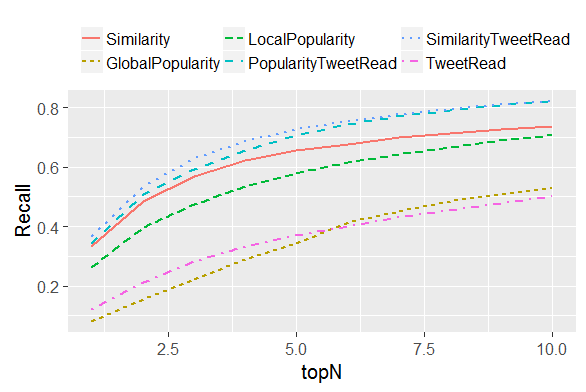
\includegraphics[width=0.48\textwidth]{comparison}
\caption{Comparison of re-ranking strategies for hashtag recommendation.}
\label{fig:comparison}
\end{figure}



For evaluating the strategies for hashtag recommendation, we used the same dataset as in the previous example, but we followed a leave-one-out strategy this time. For each tweet, top N hashtag recommendations were computed. Recall measure was used to evaluate performance, determining with it to what extend where the correct hashtags recommended in the top N.

As it can be seen in Figure \ref{fig:comparison}, even if readability by its own is not a good re-ranking strategy, it is a good complement to other strategies, improving the results when combined with both popularity and similarity metrics.





 assessment of hashtag recomendation, table comparison each metric\\

\section{Conclusion and Future Work}
In this paper we presented TweetRead a novel readability assessment tool specifically designed to predict the readability of tweets. In addition, we performed an initial study to demonstrate the benefit of using a readability signal in the hash-tag recommendation task with promising results.

In the future, we plan to explore other applications of readability in social networks, such as user recommendation, advertisement targeting or re-tweet prediction. We will also explore techniques to further enhance TweetRead and adapt it to other social networks beyond Twitter.

%
% The following two commands are all you need in the
% initial runs of your .tex file to
% produce the bibliography for the citations in your paper.
\bibliographystyle{abbrv}
\bibliography{sigproc}  % sigproc.bib is the name of the Bibliography in this case
% You must have a proper ".bib" file
%  and remember to run:
% latex bibtex latex latex
% to resolve all references
%
% ACM needs 'a single self-contained file'!
%

\end{document}
